Our goal is to infer the probability of each neuron spiking at any time, conditioned on \emph{all} the fluorescence measurements from the entire population of neurons: $\p(\bn_t | \bF_{1:T})$ for $t = 1. \ldots, T$.  As the uncertainty is non-Gaussian (due to the assumed Bernoulli distribution governing spikes), and the dynamics are nonlinear (due to the saturation of fluorescence, $S(\cdot)$, standard linear-Gaussian filtering is inadequate for this model.  Instead, we generalize our previous result \cite{BJ08}, in which we utilized sequential Monte Carlo methods to develop a model-based optimal nonlinear filter.  Very briefly, in that work, we used a particle filter to recursively infer $\p(n_t | F_{1:t})$, for $t=1, \ldots, T$, and used a particle smoother to recurse backwards, obtaining $\p(n_t | F_{1:T})$ \cite{DoucetGordon01}.  By embedding this particle-filter-smoother (PFS) into an expectation-maximization framework, we can iterate inferring the hidden spike trains and learning the parameters \cite{DoucetGordon01}.  Importantly, in that work, we modeled each neuron as an independent generalized linear model (GLM).  In contrast, here we model the neurons as coupled GLMs \cite{Paninski04c, TruccoloBrown05, Pillow08}.  Thus, we can condition the probability of each neuron spiking at any time on the spike history of all observed neurons. More precisely, we proceed as described in Algorithm \ref{alg:1}.  Note, we have assumed that all the parameters governing $\bF$ and $\bC$ have been estimated already, using the GLM PFS described in \cite{BJ08}.

\begin{algorithm}
\caption{Pseudocode for inference and learning for a population of simultaneously observed neurons.  } \label{alg:1}
\begin{algorithmic}[1]
\WHILE[$j$ indexes iterations]{$j=1, \ldots$} 
\FOR[$i$ indexes neurons]{$i=1$ to $m$}
\STATE Let $\tbx_{i,t}^{(j)}=\big[\bx_t,\: \tbh_{\backslash i,t}^{(j)}\big]'$, where $\tbh_{\backslash i, t}^{(j)}=E[\bh_{\backslash i,t}^{(j)} | \bF_{1:T}]$ and $\bh_{\backslash i,t}=\{h_{1,t}, \ldots, h_{i-1,t}, h_{i+1,t}, \ldots, h_{m,t}\}$
\STATE Let $\tbk_i^{(j)}=\big[\bk_i^{(j)},\: \ve{\omega}_{\backslash \bi}^{(j)}\big]'$, where $\ve{\omega}_{\backslash \bi}=\{\omega_{i,1}, \ldots, \omega_{i,i-1}, \omega_{i,i+1}, \ldots, \omega_{i,m}\}$
\STATE Infer $P_{\bth^{(j)}} (\{C,n,h\}_{i,t}^{(j+1)} | \bF_{1:T}) \: \forall t$ where $n_{i,t} \sim $ Ber$\big(n_{i,t}; \big(\tbk_i^{(j)}\big)' \tbx_{i,t}^{(j)}\big)$ using GLM PFS as described in \cite{BJ08}
\ENDFOR

\FOR{$i=1$ to $m$}
\STATE  Estimate $\tbk_i^{(j+1)}=\big[\bk_i^{(j+1)}, \: \ve{\omega}_{\backslash \bi}^{(j+1)}\big]$ using GLM PFS as described in \cite{BJ08}
\ENDFOR

\ENDWHILE
\end{algorithmic} 
\end{algorithm}

\begin{figure}[h!] 
\begin{center} 
%\epsfxsize=4.4in 
%\epsfysize=2.4in \epsffile{SimConnector.eps} 
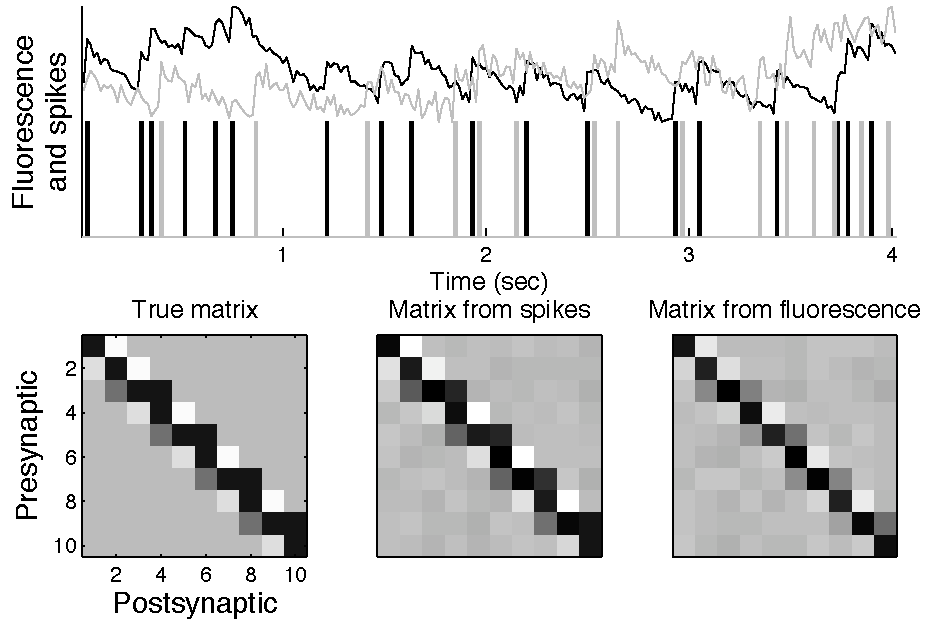
\includegraphics[width=0.7\linewidth]{../figs/SimConnector} 
\caption{Inferring network connectivity given noisy simulated calcium fluorescence data. Our main result is that we can infer network connectivity given only short sequences of observations ($<10$ min), for small populations of neurons ($\sim 10$), given reasonable assumptions on spike rate ($\sim 5$ Hz), observation frequency ($60$ fps), and observation noise. \textbf{Top}: True spikes and observed noisy calcium fluorescence traces for two cells in the simulated network.  Calcium data sampled at 60 Hz.  (Only four seconds of a longer experiment are shown here, for clarity.)  \textbf{Bottom}: True connectivity matrix; connectivity matrix estimated given the fully observed spikes; and connectivity matrix estimated given just the noisy calcium data, given about 2000 spikes/neuron.  White denotes excitatory connections; black denotes inhibition; the same grayscale map is used for each panel.  A small simulated network was used for illustration purposes.  Each cell inhibited itself following each spike (a relative refractory effect) and excited or inhibited its nearest neighbors; the strength and time constant of these excitatory terms were chosen to mimic the experimentally determined parameters (a spike in one cell modulates the instantaneous firing rate in another cell by no more than $5\%$ -- $10\%$).  No external drive was applied to the network; i.e., only spontaneous network dynamics are observed here.  Note that it is somewhat harder to estimate the connectivity map given noisy calcium data than the true spike trains (specifically, some of the inhibitory connections are slightly underestimated in the right panel); nonetheless the correct connectivity is obtained with only a few minutes of calcium data.} \label{fig:gibbs} 
\end{center}
\end{figure}
